\documentclass[a4paper, 11pt, oneside]{article}

\newcommand{\plogo}{\fbox{$\mathcal{PL}$}} 
\usepackage{amsmath}
\usepackage[utf8]{inputenc} 
\usepackage[T1]{fontenc} 
\usepackage{enumitem}
\usepackage{graphicx}
\usepackage{graphicx}
\usepackage{supertabular}
\usepackage{hyperref}
\usepackage[spanish]{babel}
\graphicspath{{Imagenes/}}

\begin{document} 

\begin{titlepage} 

	\centering 
	
	\scshape 
	
	\vspace*{\baselineskip} 
	
	
	
	\rule{\textwidth}{1.6pt}\vspace*{-\baselineskip}\vspace*{2pt} 
	\rule{\textwidth}{0.4pt} 
	
	\vspace{0.75\baselineskip} 
	
	{\LARGE Practica 5}	
	\vspace{0.75\baselineskip} 
	
	\rule{\textwidth}{0.4pt}\vspace*{-\baselineskip}\vspace{3.2pt}
	\rule{\textwidth}{1.6pt} 
	
	\vspace{2\baselineskip} 
	

	ADMINISTRACIÓN DE SISTEMAS UNIX/LINUX
	
	\vspace*{1\baselineskip} 
	
	
	
	Alumnos:
	
	\vspace{0.2\baselineskip} 
	
	{\scshape\Large Karla Adriana Esquivel Guzmán url{https://github.com/karlycaramelo} \\
    Eric Giovanni Miguel Torres url{https://github.com/EricGiovanni}\\ 
    María Ximena Lezama Hernández url{https://github.com/LezamaXi}\\ 
    Gonzalo Vazquez Cruz url{https://github.com/truerandom}}  
	\vspace{0.5\baselineskip} 
	\vfill
	
\includegraphics{unam.jpg}
	
	\textit{UNIVERSIDAD NACIONAL AUTONOMA DE MEXICO} 
	
	
	
	
	
	\vspace{0.3\baselineskip} 
	
	22/Febrero/2019 
	
	 

\end{titlepage}
\begin{itemize}
    \item Lo primero que hicimos fue configurar una red en VirtualBox.
    \begin{center}
    
\includegraphics[scale=0.40]{1.png}    
    \end{center}
    
    \item Configuramos nuestra maquina virtual de windows y al NAT Network le asignamos la red de VirtualBox.
    
    \begin{center}
    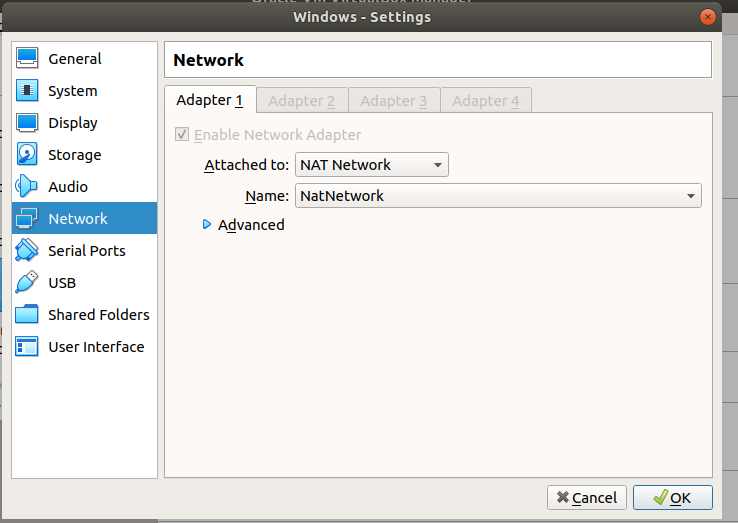
\includegraphics[scale=0.40]{2.png}    
    \end{center}
    
    
    \item Configuramos el Bridge y la NAT Network a la que le asignamos la red de VirtualBox, esto para la maquina virtual de Debian.
    
    \begin{center}
    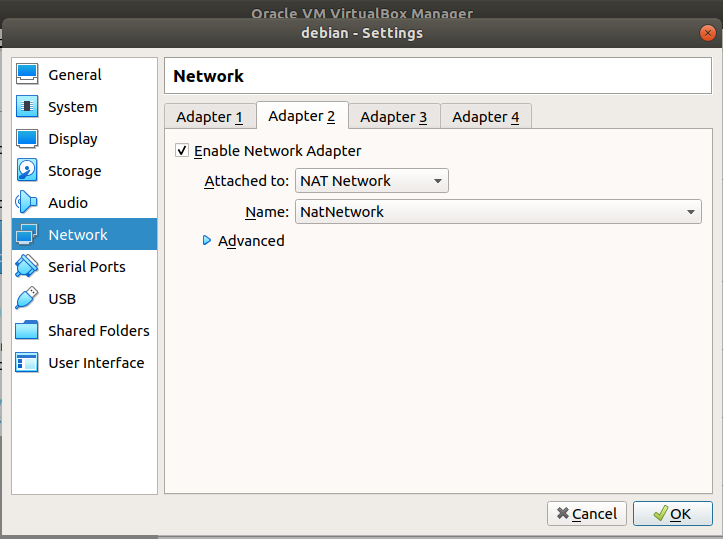
\includegraphics[scale=0.40]{3.png}    
    \end{center}
    
    
    \item Instalamos \textbf{Samba} en Debian con el comando apt-get install samba cifs-utils.

    
    
    \item Posteriormente configuramos Samba y creamos la carpeta que se quiere compartir, es importante que a esta carpeta se le den los permisos de libre acceso, puesto que de otra manera la carpeta no puede ser accesada desde Windows.
    
    \begin{center}
    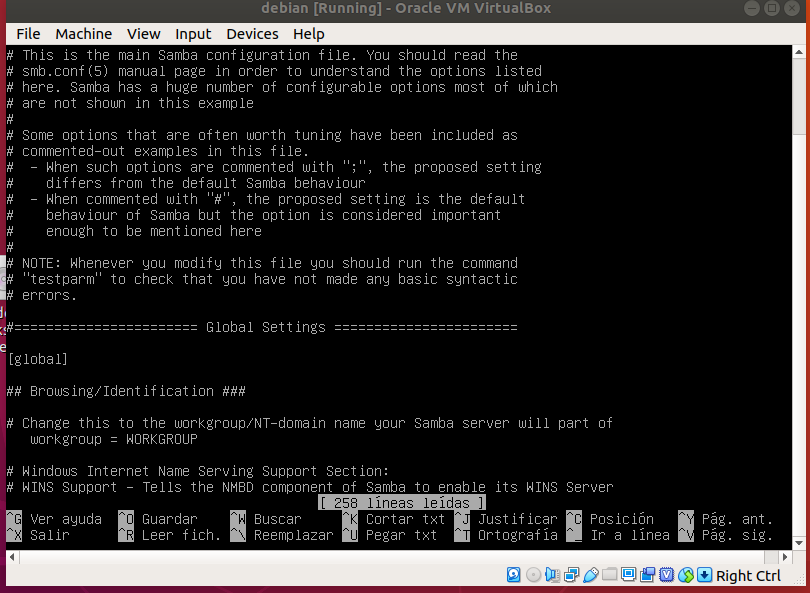
\includegraphics[scale=0.40]{4.png}    
    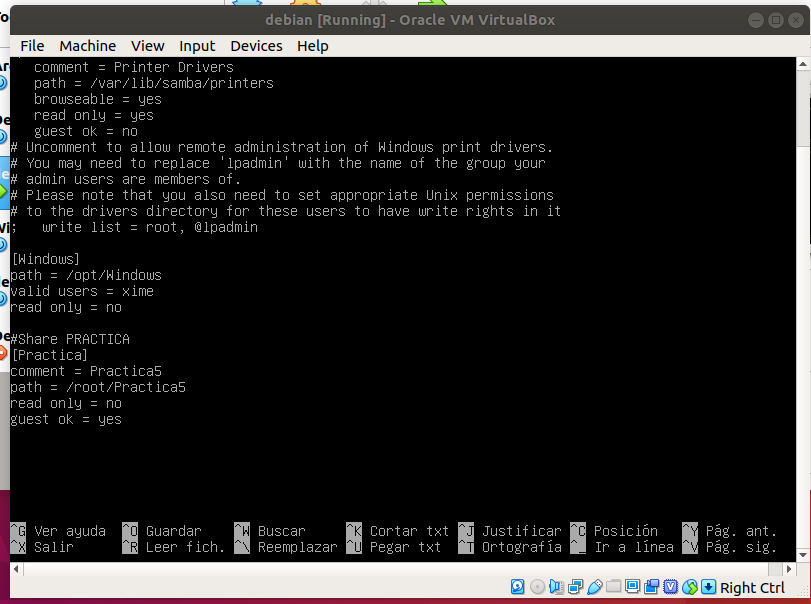
\includegraphics[scale=0.40]{5.png}
    \end{center}
    
    \item Para que podamos tener acceso a Debian desde Windows, configuramos el protocolo $SMB 1.0/CIFS$ en Windows.
    
    \begin{center}
    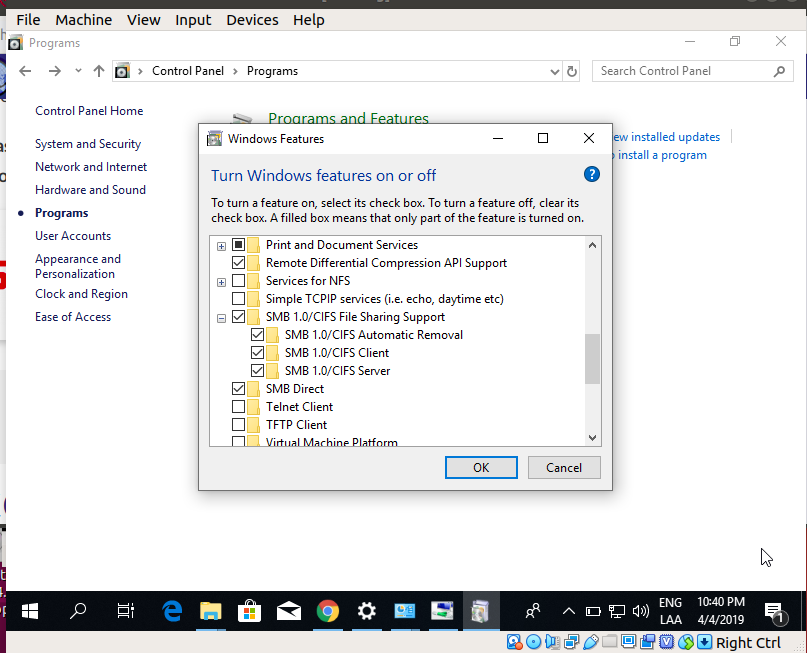
\includegraphics[scale=0.40]{6.png}    
    \end{center}
    
    \item Por último si todo está correcto, aparecerá la carpeta compartida dentro de Network.
    
    \begin{center}
    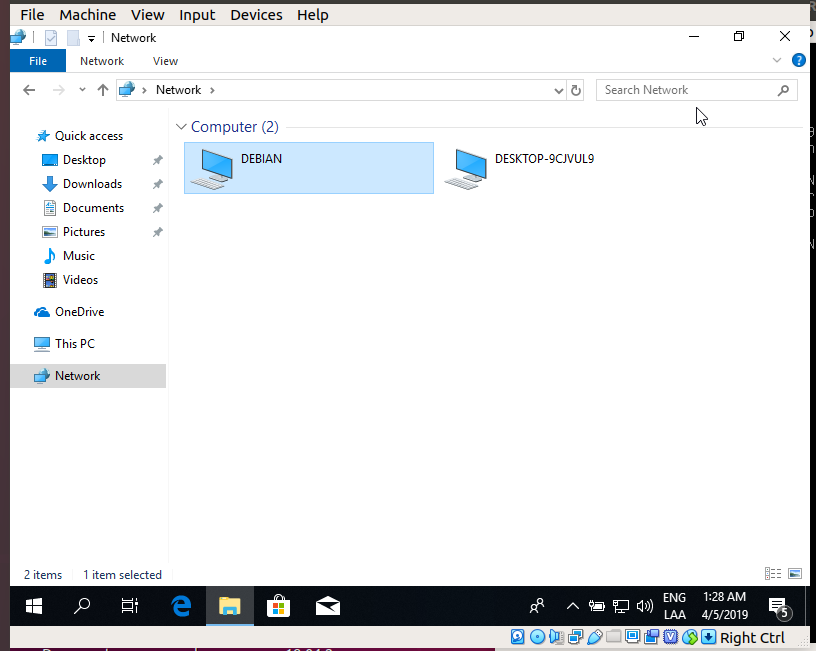
\includegraphics[scale=0.40]{7.png}
    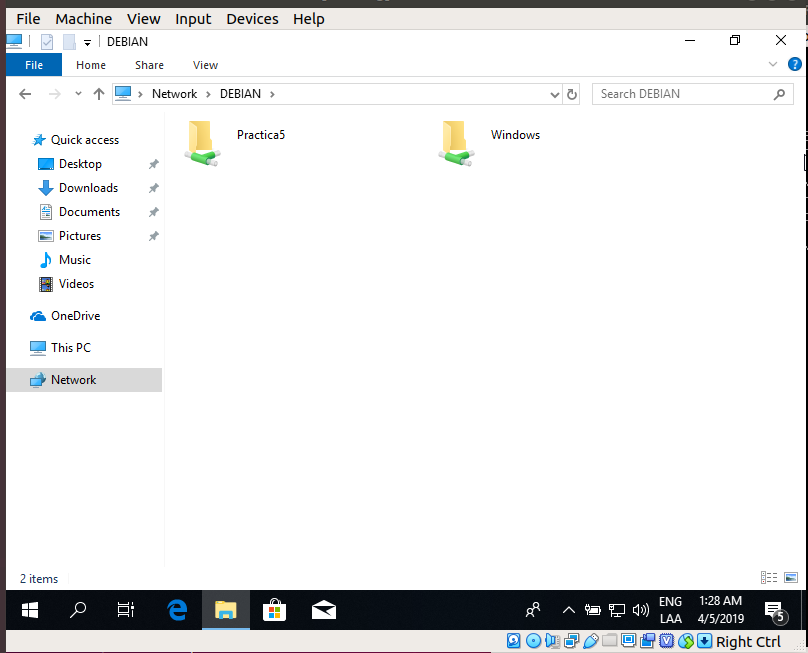
\includegraphics[scale=0.40]{8.png}
    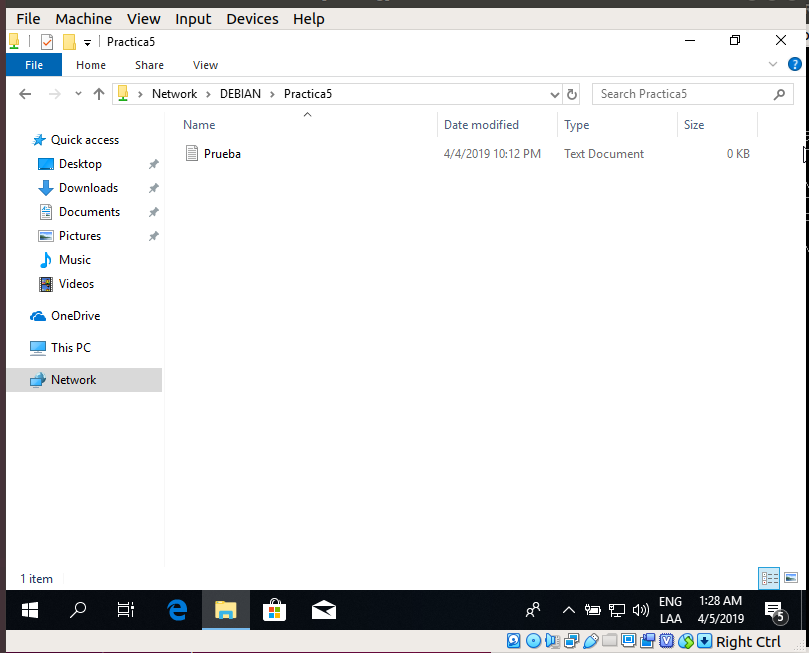
\includegraphics[scale=0.40]{9.png}
    \end{center}
\end{itemize}
\end{document}